\chapter{Le \emph{Journal Officiel} : la parole, la main, la vue et le droit}

\enquote{Pas de question sans document. [La question de l'historien] n'est pas une question nue; c'est une question armée, qui porte avec elle une idée des sources documentaires et des procédures de recherches possibles}. \footcite[][80]{prost}. Ainsi, Antoine Prost, à partir des propositions de Robin G. Collingwood sur les questions historiques, expose l'idée d'une solidarité entre une question de recherche, les documents et les procédures de leur traitement. La question de l'historien, tout d'abord, est \enquote{armée} : cela signifie qu'elle ne vient pas seule pour satisfaire, avec désintéressement, une curiosité passagère; elle prend appui sur l'actualité de l'historien, de ce qui fait qu'elle puisse être pertinente socialement et scientifiquement. \enquote{Armée} : cela veut dire également que l'historien a déjà une idée des sources documentaires sur lesquelles travailler. Le chemin de la connaissance du passé, qui s'ouvre avec une question de recherche, est motivé par un \emph{reenactement}, une réactivation du passé depuis le présent. Par là, il s'agit d'être à l'écoute des \enquote{palpitations du temps} présent -- pour reprendre ce mot de l'historien de l'art Eugeni d'Ors \footcite[][]{ors} -- et de réinterroger l'actualité à travers des documents à explorer. \enquote{Il n'y a d'histoire que de choses pensées au présent par l'historien}\footcite[][p.166]{prost} : selon l'approche collingwoodienne -- qui n'est d'ailleurs pas sans rappeler la position de Walter Benjamin sur l'histoire comme \enquote{objet d’une construction dont le lieu n’est pas le temps homogène et vide, mais qui forme celui qui est plein de temps actuel} \footcite[][]{benjamin} -- la pratique historienne est une dialectique entre passé et présent. Les documents, alors, ne sont pas \enquote{un dépôt mort} mais une \enquote{énergie fossile} qui reffectue une pensée\footcite[][]{libera} et viennent renouveler un questionnaire. Les prétentions historiennes collingwoodiennes semblent alors aller au-delà d'une satisfaction strictement érudite -- ou du moins sans volitions éthiques -- pour atteindre la nécessité de réévaluer le passé avec des considérations toutes pragmatistes, c'est-à-dire valuatives\footcite[][]{dewey}. Si l'historien est lui-même un sujet situé historiquement et socialement, il est également saisi dans des configurations techniques qui peuvent changer ses procédures de recherche -- la numérisation de sources historiques et leur mise à disposition sur le Web étant un exemple assez criant. Le milieu de l'historien a donc lui-même une historicité; sociale, technique, psychique --  car \enquote{il n'y a pas d'histoire sans préjugés} selon les mots de Francis H. Bradley, rapportés par Antoine Prost\footcite[][p. 96]{prost}.

À l’heure où la question de la dette occupe le centre des débats publics, il est pertinent de réactiver une pensée historique pour éclairer les inquiétudes du présent. L’analyse des débats parlementaires d’autres périodes de crise, saisis à travers le \emph{Journal officiel} et des instruments de repérage comme les tables nominatives, offre une occasion de réfléchir à la qualité des échanges démocratiques et aux formes de polarisation politique qui traversent nos institutions. Ainsi, les controverses actuelles sur \enquote{l’ensauvagement} du débat parlementaire\footcite[][]{ensauvagement}, ou encore sur la \enquote{polarisation}\footcite[][]{polarisation} politique française dans un cadre international sous tension, ne se comprennent pleinement que replacées dans une histoire longue des pratiques délibératives et des dynamiques institutionnelles. Le \emph{Journal officiel}, qui restitue l'activité parlementaire, accompagne donc la question de la polarisation politique. Ce travail engage à une double exigence : d’une part, saisir la singularité des crises d’hier -- comme celles économiques de 1931 -- dans leurs propres rationalités politiques et sociales ; d’autre part, réfléchir aux continuités et ruptures qui relient ces débats à notre époque, à travers la médiation des sources et des techniques de recherche actuelles. Le \emph{reenactment} collingwoodien prend ici toute sa portée : relire le passé n’est pas reproduire mécaniquement des faits, mais réactualiser une pensée inscrite dans les documents avec les nouvelles opportunités techniques d'exploration des sources pour nourrir un questionnement critique sur le présent.

Dans cette partie, cette question de la polarisation se fait point de départ pour une investigation sur les procédures techniques d’exploration des sources sérielles. Si la question historienne est aussi un dialogue avec des sources, elle est également médiatisée par les méthodes employées pour les interroger et par les relations qu’elles peuvent tisser entre elles. Il faut donc comprendre \emph{comment} la source est fabriquée, ce qu’elle est capable de restituer ou, au contraire, de rendre absent ; analyser également sa place dans un « énoncé »\footcite[][]{Foucault}, en interrogeant sa position disciplinaire -- les numéros du \emph{Journal Officiel} sont des archives ou de la documentation ? Qu'est-ce que cette classification peut dire de son rôle ? -- ; et enfin étudier son fonctionnement prosaïque, c’est-à-dire saisir l’écologie documentaire dans laquelle est s'inscrit. Nous commencerons par dessiner une histoire synthétique de la transcription des débats parlementaire et de l'édition des lois publiées -- du \emph{Moniteur universel} au \emph{Journal Officiel} en passant par \emph{Le Bulletin des lois} -- puis nous donnerons plus d'attention au \emph{Journal Officiel} dans les années 30, à partir des archives de la \emph{Direction du Journal Officiel}, administration du Ministère de l'Intérieur.

\section{Le \emph{Journal Officiel} : le droit et la main}

Le \emph{Journal Officiel} est l’aboutissement d’une longue évolution des supports de publicisation des débats parlementaires et des textes législatifs en France. S'il né en 1869, sous le Second Empire, c'est en remplacement du \emph{Moniteur universel}, lui-même héritier des ambitions révolutionnaires. Son histoire reflète cependant une transformation plus large : celui du passage d’une logique où la transparence des débats publics à l'Assemblée nationale était un idéal politique à une ère où la publication des textes législatifs devient un acte juridique fondateur. Cette métamorphose, qui s’étend sur plus de deux siècles, illustre le passage d’une logique de transparence, forgé par un idéal politique révolutionnaire; à une ère où la publication devient un acte performatif, indissociable de la validité des textes législatifs.

\subsection{La Révolution française : l’émergence d’une publicité politique (1789–1799)}

La Révolution française marque une rupture radicale en érigeant la publicité des débats en principe constitutionnel. La Constitution de 1791 proclame ainsi que \emph{« les délibérations du Corps législatif seront publiques, et les procès-verbaux de ses séances seront imprimés »}\footcite[][]{constitution} actant la nécessité de rendre compte au peuple des discussions qui engagent son destin. Cette exigence de transparence se concrétise par la création de deux organes distincts, répondant à des logiques complémentaires mais distinctes : le \emph{Moniteur universel}, initiative privée -- et le \emph{Bulletin des lois} -- initiative du Directoire qui, selon Frédéric Graber, a servi à \enquote{forcer le consentement} des citoyens à la loi \footcite[][]{graber}. 

Le \emph{Moniteur universel}, fondé en 1789 par Charles-Joseph Panckoucke, s’impose rapidement comme le premier vecteur de publicisation des débats parlementaires et qui connut un \enquote{vif succès public} car produisant \enquote{un fort effet de réel} \footcite[][]{coniez}. Son ambition affichée est de retranscrire les discussions de l’Assemblée nationale, mais ce travail de transcription, loin d’être neutre, relève déjà d’une reconstruction orientée. Comme le souligne Benjamin Morel, ces comptes rendus n’étaient pas de simples \emph{verbatims} : ils reflétaient les lignes de force politiques de l’époque, tout en servant un objectif plus large, celui de rendre publique une parole parlementaire en construction. Par exemple, les journalistes du \emph{Moniteur}, comme Hugues-Bernard Maret, devaient résumer ou interpréter les propos en fonction de leurs affinités politiques, mais aussi des contraintes techniques de l’époque\footcite[][]{coniez}. Les débuts de la transcription étaient en effet artisanaux : les rédacteurs prenaient des notes à la main, ce qui rendait les comptes rendus souvent incomplets ou biaisés. Dès l’origine, il s’agissait de produire un texte lisible, adapté à un public élargi, tout en servant les intérêts d’une institution en quête de légitimité\footcite[][]{morel}. Une innovation notable fut le \emph{Journal logographique} (1791), créé par Le Hodey de Saultchevreuil, qui utilisait une méthode de rotation entre plusieurs rédacteurs pour capturer l’intégralité des débats, utilisant un système de bande de papier étroites et allongées. Chaque \enquote{logographe} prenait des notes pendant quelques minutes avant de passer le relais, permettant une couverture plus complète. Cependant, cette méthode, bien qu’ingénieuse, échouait à restituer la plurivocité des échanges, réduisant la complexité des débats à une succession de discours linéaires\footcite[][]{coniez}.

Parallèlement, le \emph{Bulletin des lois}, créé en 1793, remplit une fonction radicalement différente. Contrairement au \emph{Moniteur}, qui se concentre sur les débats, le \emph{Bulletin} a pour vocation exclusive de publier les lois et décrets adoptés par les assemblées révolutionnaires\footcite[][]{saudrais}. Son objectif n’est pas d’informer ou d’éduquer, mais de rendre opposables les textes législatifs en les portant à la connaissance des citoyens et des autorités locales. La publication est un relais d’information législative puis, sous le Directoire, un acte fondateur de la validité juridique : une loi non publiée n’existe pas en droit. Cette distinction fondamentale entre les deux organes – l’un tourné vers la délibération, l’autre vers la norme – préfigure la dualité fonctionnelle qui caractérisera plus tard le \emph{Journal Officiel}. 

Ainsi, dès ses origines, la publicisation des débats et des textes législatifs répond à deux logiques distinctes, voire antagonistes : une logique démocratique, où la transparence vise à éclairer le citoyen et à légitimer le pouvoir par le débat ; et une logique juridique, où la publication conditionne l’effectivité des normes. Ces deux dimensions, bien que coexistantes, restent cependant séparées jusqu’au milieu du XIXe siècle.

\subsection{Le XIXe siècle : vers une institutionnalisation de la transparence (1800–1870)}

Au cours du XIXe siècle, les régimes successifs – Consulat, Empire, Restauration, Monarchie de Juillet, Seconde République – maintiennent une publicité contrôlée des débats parlementaires, mais deux évolutions majeures se dessinent, qui vont progressivement rapprocher les fonctions de publicisation et de légalisation. D’une part, la professionnalisation des comptes rendus, avec la professionalisation de la sténographie et ses méthodes de retranscription plus fidèles et systématiques des débats\footcite[][]{gardey}. D’autre part, la fusion progressive des organes de publication prépare le terrain à l’émergence d’un support unique, combinant les héritages du \emph{Moniteur} et du \emph{Bulletin des lois}.

Sous le Consulat et l’Empire, le \emph{Moniteur universel} perd son indépendance pour devenir un organe de propagande au service du pouvoir napoléonien\footcite[][]{universalis}. Les comptes rendus y sont épurés, voire censurés, et la transparence n’y est plus un idéal démocratique, mais un instrument de légitimation du régime. Cette période marque un recul temporaire dans la publicisation des débats, mais elle ne remet pas en cause la nécessité structurelle de rendre compte, ne serait-ce que de manière contrôlée, des travaux parlementaires. 

La Restauration et la Monarchie de Juillet voient cependant un renouveau de la publicité parlementaire, porté par deux dynamiques complémentaires. D’une part, les progrès techniques, sous l'impulsion des services de sténographie des chambres d'un Prévots et d'un Célestin Lagache, permettent une retranscription plus précise des débats\footcite[][]{coniez}. En 1831, Jean-Baptiste Breton fonde le \emph{Sténographe des Chambres}, première tentative de compte rendu intégral fondé sur une méthode systématique de prise de notes\footcite[][]{coniez}. Bien que cette initiative échoue faute de moyens -- car sa méthode sténographique impliquait un dispositif couteux, basé sur la relève régulière des sténographes, chacun étant une tête à rémunérer --, elle préfigure la professionnalisation des rédacteurs parlementaires. D’autre part, la montée en puissance des assemblées sous la Monarchie de Juillet conduit à une demande croissante de transparence. En 1848, l’Assemblée nationale intègre les sténographes dans ses services, marquant la naissance d’un corps de fonctionnaires dédiés à la retranscription des débats. Le compte rendu cesse d’être une initiative privée pour devenir un document officiel, garanti par l’État. la révolution dans la transcription des débats parlementaires est venue avec le développement de la sténographie. Si cette technique, introduite en France à la fin du XVIIIe siècle, consistait à utiliser des signes abrégés pour noter la parole à la vitesse à laquelle elle était prononcée, la sténographie n’était pas seulement un outil technique, mais un instrument politique : elle permettait en effet de transformer une parole orale, souvent chaotique, en un discours écrit structuré, parfois conforme aux attentes d’un État en quête d’ordre et de rationalité\footcite[][]{morel}. Avec l'intègration officielle des sténographes dans les services parlementaires, vient à naître un corps de sténographes d’État. Cette institutionnalisation répondait à un double impératif : assurer la publicité des débats -- un principe constitutionnel -- et contrôler la production du compte rendu pour en faire un outil au service de la légitimité parlementaire.  Cette institutionnalisation s’accompagne donc d’une codification stricte des méthodes de rédaction. Les sténographes, désormais soumis à des règles précises, ne se contentent plus de transcrire, mais recomposent les discours pour les adapter aux exigences de la langue écrite et aux attentes d’un lectorat élargi. Comme l’a souligné Hippolyte Prévost, leur travail relève moins de la transcription littérale que de la traduction : il s’agit de « rendre justice à l’orateur » tout en produisant un texte « clair, cohérent et conforme aux canons de l’écrit » \footcite[][]{morel}. Cette approche, qui privilégie la lisibilité à la fidélité absolue, sera reprise et systématisée par les services officiels du \emph{Journal Officiel}. Pallèlement, le \emph{Bulletin des lois} poursuit sa mission de publication des textes normatifs, mais son rôle se trouve progressivement absorbé par celui du \emph{Moniteur}, qui, sous la Seconde République, commence à intégrer des extraits législatifs. Cette convergence prépare le terrain à la fusion des deux fonctions – information et légalisation – qui interviendra à la toute fin du Second Empire.

La création du \emph{Journal officiel de l’Empire français} en 1869, sous Napoléon III, marque un tournant décisif. Pour la première fois, un seul organe rassemble les débats parlementaires, héritiers du \emph{Moniteur universel}, et les lois et décrets, héritiers du \emph{Bulletin des lois}. L’adjudication du 24 septembre 1868, publiée dans le \emph{Journal officiel} du lendemain, attribue « le droit exclusif d’imprimer et de publier les deux journaux officiels paraissant sous le titre de \emph{Moniteur universel} » à l’imprimeur Wittersheim au 31 quai Voltaire à Paris, à proximité du Sénat et du Corps législatif -- la publication comprenant également l'envoi à la poste et la désignation des \enquote{écrivains} étant une prérogative gouvernementale\footcite[][]{cote1}. L'adjudicataire sera ainsi tenu de \enquote{publier chaque jour [...] les comptes rendus sténographiques des séances du Sénat et du Coprs législatif, les lois, décrets et actes officiels, judiciaires ou administrative dont l'insertion est réclamée par le Gouvernement}\footcite[][]{cote1}. Ce texte place celui-ci sous la tutelle du ministre Ernest Pinard, soumet la désignation des rédacteurs à l’approbation de l’exécutif et prévoit que, en cas de manquement, le contrat peut être résilié par voie de régie\footcite[][]{cote1}, sous les douze ans. Le premier numéro sera publié le 1er janvier 1869 sous le nom de \emph{Journal Officiel de l'Empire français} et sera renommé en 1870 \emph{Journal Officiel de la République française} à la chute du régime impérial. En 1870 commence réellement une transition administrative et organisationnelle, suite à l'instabilité politique et la guerre -- l'envoi du \emph{Journal Officiel}, pendant le siège de Paris de 1871 sera d'ailleurs envoyé expédié par ballon; les bureaux et imprimerie déménagés à Tours sous la Délégation du Gouvernement de la Défense Nationale puis à Versailles jusqu'en 1879\footcite[][]{cote1}. En 1880, avec la loi du 28 décembre, est créée l'administration du \emph{Journal Officiel}, placée sous la tuelle du Ministère de l'Intérieur. C'est une société anonyme de composition -- la SACIJO, (Société Anonyme de Composition et d'Impression du \emph{Journal Officiel}) -- qui sera en charge de l'impression.

Cette fusion des comptes rendus et publication des actes officiels n’est pas anodine : elle signe en fait la réconciliation des deux logiques qui, depuis 1789, coexistaient sans se confondre. Désormais, la publicisation des débats et la publication des textes normatifs ne sont plus deux missions distinctes, mais les deux faces d’une même entreprise : éclairer le citoyen tout en fondant la légalité des actes. Avec la chute du Second Empire et l’avènement de la IIIe République en 1870 --- le journal devenant le \emph{Journal officiel de la République française} -- consacre une nouvelle ère dans l’histoire de la publicité parlementaire. 

\subsection{L'organisation du \emph{Journal Officiel} au XXe siècle}

Un rapport du directeur Pierre Cassagneau du 11 juillet 1945, adressé au Conseiller d'Etat du Gouvernement Provisoire, nous renseigne sur l'organisation historique du \emph{Journal Officiel} qu'il dirige \footcite[][]{cote6} : depuis la direction du Ministre Fallières de 1881, l'organisation reste globalement la même, si l'on fait abstraction du nombre des employés de l'administration et des ouvriers de la SACIJO pouvant varier. La Direction du \emph{Journal Officiel} se compose de cinq services : celui de la rédaction; de la caisse de comptabilité; de la gestion du matériel; de la vente et des abonnements; et enfin le service de la correspondance et des Tables. Le personnel se compose alors notamment d'un Directeur -- nommé par décret \footcite[][]{cote1} --, de secrétaires, de caissiers, de comptables, de mécaniciens, d'imprimeurs. Les services administratifs ont pu bénéficier en 1909 d'un statut de fonctionnaires titulaires; quant aux services dits ouvriers -- les clicheurs, linotypistes, rotativistes, etc. -- ils sont organisés de façon similaire à une coopérative ouvrière de production, car elle comprend des ouvriers actionnaires\footcite[][]{cote6}. Le rapport de Pierre Cassagneau mentionne également une organisation complexe (voir \ref{fig:organigramme}), entre la gestion des envois; la comptabilité des nombreuses opérations d'impression du \emph{Journal}; les services d'entretien du matériel et des locaux; l'augmentation du courrier à gérer --  plus de 30000 lettres par an --; l'approvisionnement du matériel et des combustibles pour l'impression -- les linotypes exigeant la fonte du plomb pour la clicherie -- l'accroissement des textes à insérer et des tirages : entre les années 1910 et 1930, la production du \emph{Journal Officiel} augmente: il y a près de 19000 abonnés en 1913 contre 34000 en 1938 et 85700 en 1945. Du côté de la rédaction, les secrétaires travaillent de jour comme de nuit et assurent des navettes entre l'imprimerie et les services sténographiques des assemblées pour veiller à la qualité des transcriptions. Quant aux ouvriers de la clicherie, exposés à la chimie de la fonte, ils travaillent dans des espaces mal aérés dans des locaux d'une quarantaine de mètres carrés au 29 quai Voltaire -- et les rotativistes dans des espaces plus grands -- 380 $m^2$ -- mais exigus pour leur tâche. On note également en 1930, puis en 1934, le \emph{Journal Officiel} une compression du personnel avec la suppression d'une dizaine de poste en même temps qu'une augmentation des abonnements et des tirages -- qui a d'ailleurs exigé, dans les années 20, l'acquisition progressive d'une trentaine de linotypes composant en \emph{Romain Dorique} pour remplacer le matériel d'impression à plat manuel.

\begin{figure}[htbp]
\centering
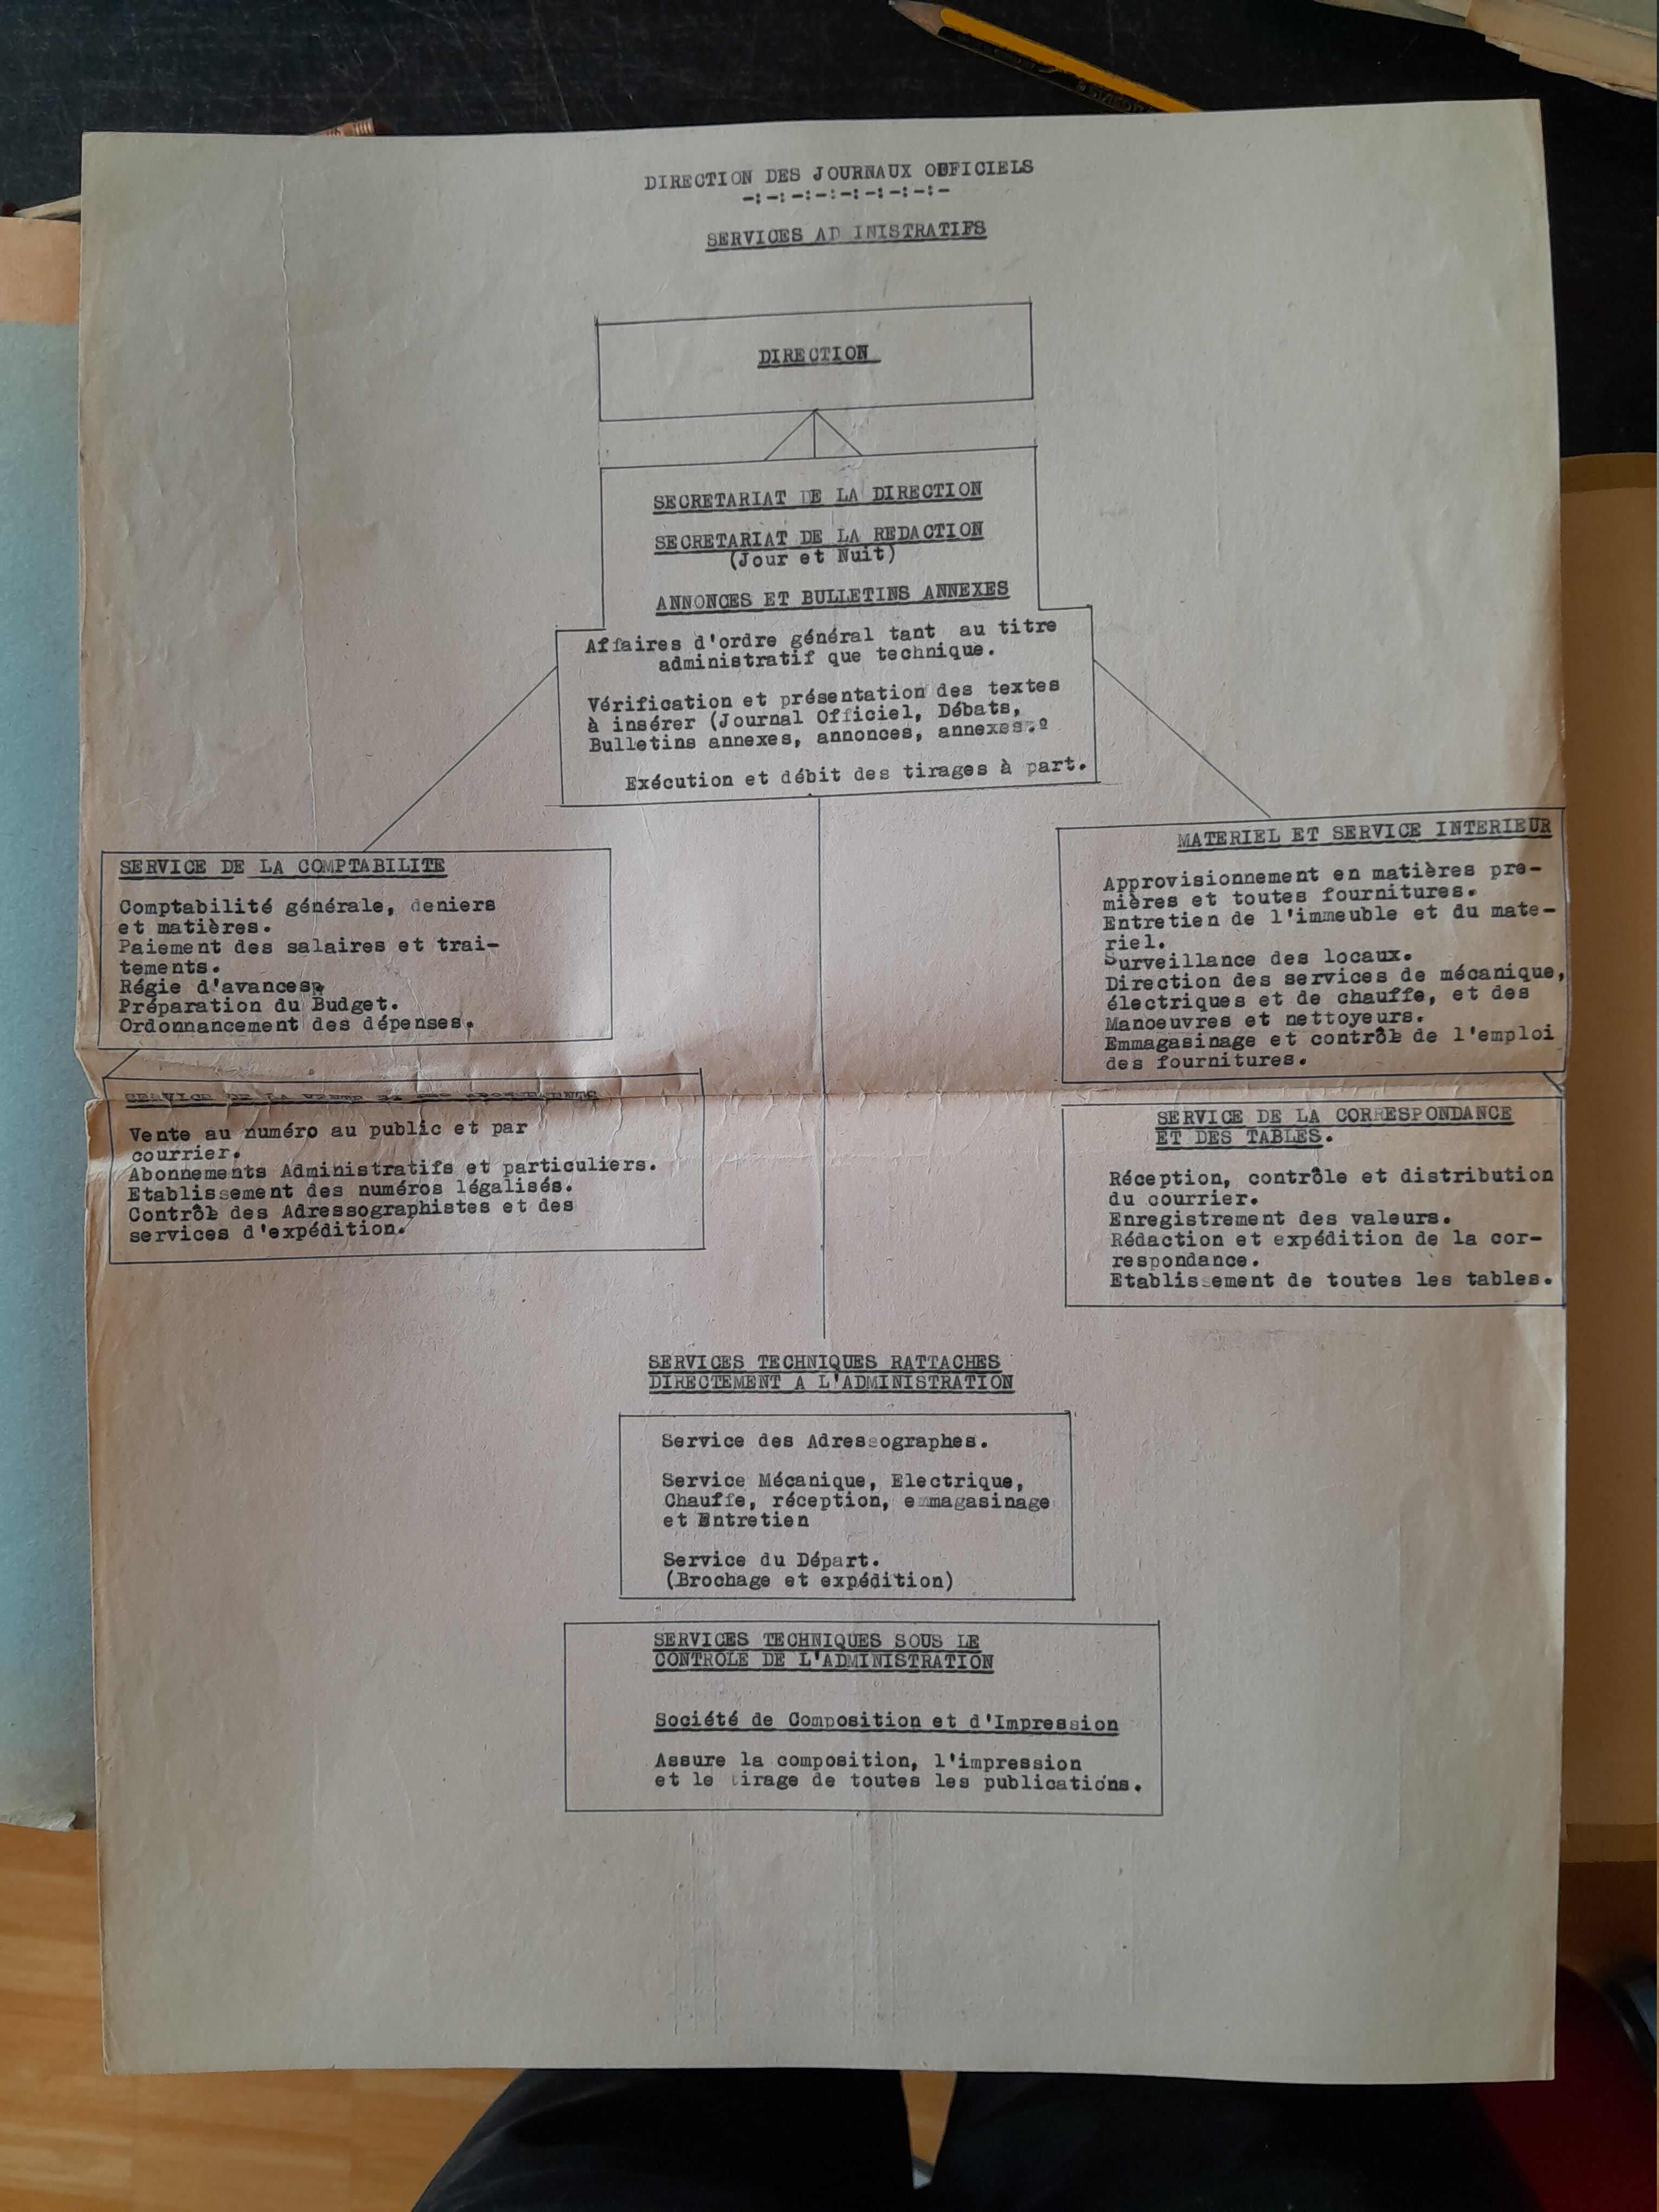
\includegraphics[width=\linewidth]{organigramme.jpg}
\caption{Archives nationales (site de Pierrefitte-sur-Seine), fonds du ministère de l'Intérieur, 19870069/6, Dossier \enquote{Organigramme et personnele} }
\label{fig:organigramme}
\end{figure}

Quant aux \emph{Tables}, elles impliquent un service propre qui a \enquote{un travail minitieux} et \enquote{l'établissement rationnel} d'un système de classement comptant près de 25000 fiches\footcite[][]{cote6}. Le service, en charge de la réalisation des tables alphabétiques mensuelles, des tables des tirages financiers, des Débats de l'Assemblée, des Documents administratifs, des questions écrites et des tables chronologiques, participe également à la lecture et la révision des épreuves. 

On le voit : entre la parole de l'orateur et la lettre imprimée, il y a tout un cheminement documentaire et technique qui implique des choix éditoriaux : quand on travaille sur une telle matière, il faut avoir en tête que ces textes sont le produit d'une chaîne technique assurés par des opérateurs de spécialités très diverses.

\section{Une histoire du \emph{Journal Officiel} par sa nature documentaire : archives ou documentation ?}

On le voit : le \emph{Journal Officiel} est une véritable entreprise éditoriale; elle exige une véritable organisation et division du travail pour restituer l'activité parlementaire. Il s’agit maintenant d’interroger sa place dans les dispositifs documentaires et archivistiques car, s'il est soumis au dépôt légal -- il est conservé à la Bibliothèque nationale de France, aux bibliothèques de l’Assemblée nationale et du Sénat, et dans les bibliothèques des Archives nationales. Cette logique de diffusion correspondrait à sa vocation première : rendre publique la loi et l’activité parlementaire, garantir leur accessibilité.

Pourtant, le \emph{Journal Officiel} occupe également une place dans les Archives départementales, au sein de la série K (« Lois, ordonnances et arrêtés »), créée en 1841 : \enquote{la série K, consacrée aux recueils des lois et publications officielles, servira de complément, pour les temps modernes, aux recueils d’édits, d’ordonnances, etc., classés dans la première subdivision de la série A}. Cette série, conçue pour rassembler les actes de l’État et les publications officielles postérieures à la Révolution, accueille non seulement les arrêtés préfectoraux, mais aussi des périodiques comme \emph{Le Moniteur universel}, le \emph{Bulletin des lois} -- puis le \emph{Journal Officiel}. Or, ce classement brouille la distinction classique entre archives (documents produits par une activité administrative et conservés comme traces) et documentation -- objets édités, destinés à la lecture publique. S’il semble naturel que des publications officielles se retrouvent en K et qu’elles cohabitent avec les arrêtés — même s’il est  surprenant d’imaginer que des fonds d’archives s’enrichissent via  l’envoi régulier de périodiques dont il ne manquerait que le bulletinage pour se croire en bibliothèque — , il y a quelque autre chose à chercher du côté de l’histoire du consentement politique.

Cette inclusion du \emph{Journal} dans la série K des Archives départementales ne relève en effet pas d’une simple logique de conservation, mais d’un héritage de stratégie délibérée de fixation et de contrôle de la parole étatique. Comme le souligne Frédéric Graber\footcite[][]{graber}, la création du \emph{Bulletin des Lois} sous le Directoire s'explique à travers le problème de l'observation de la loi. La loi peut être votée et promulguée : elle ne peut obliger que si elle peut être connue de tous. Pour qu’elle soit donc connue de tous et oblige chaque citoyen, la \emph{publication} est donc nécessaire. Il faut \emph{rendre public}, c’est-à-dire \emph{confronter} les citoyens au droit. L’obligation exige l’information : "la formalisation de la publication des lois est l’œuvre cumulée des régimes successifs qui […] ont entrepris de limiter le rôle des 
administrations locales dans le processus de publication de la loi. […] La loi peut être rendue obligatoire sans avoir à la montrer effectivement aux citoyens par l’affiche"\footcite[][]{graber}. En effet, au début de la Révolution les lois étaient publiées via l’affichage -- dont avait la charge les administrations locales -- et par les crieurs publics. Or, cela  offraient aux administrations locales une plus grande agentivité: en  effet, on pouvait \emph{ne pas} afficher ou retarder l’affichage — ce  qui revient à saboter la confrontation des citoyens au droit et donc de son exécution effective — quand ce n’était pas tout simplement des problèmes techniques d’acheminement ou de réalisation des (ré-)impressions sur place. L’administration peut se montrer effrontée. Ou en tout cas pas  toujours coopérative avec le pouvoir central. Si bien que ce genre de problèmes récurrents a conduit à justifier des approches de publication plus centralisées. Un rapport du 28 brumaire an II (novembre 1793) de Billaud-Varenne, dans un contexte anti-fédéraliste où l’on accuse les administrations  départementales de faire de l’obstruction, dénonce « l’interposition des  autorités secondaires ». Suite à ce rapport, la Convention adoptera en décembre (plus précisément le 14 frimaire an II), un décret sur le mode de gouvernement provisoire et révolutionnaire : il crée le \emph{Bulletin des lois de la République}, envoyé à chaque commune par la poste. L’importance de l’affichage public, qui n’est pas vraiment remplacé, sera minoré; les marges de manœuvre des administrations départementales également.

La publication du \enquote{certifié conforme} \emph{Bulletin}, imprimé et envoyé depuis Paris ne fait cependant pas tout à fait office de promulgation, ou en tout cas pas à elle seule. Il y a toujours une proclamation orale de la loi dans les communes et la promulgation est dépendante de cette modalité d’information. Le \emph{Bulletin} est une « \emph{notification aux autorités constituées »} : elle est donc un document reçu par les administrations pour qu’elles puissent rendre publique le droit — ce sont leurs  prérogatives — et cela sans passer par le discrétionnaire des agents au  niveau départemental. Ici, on a donc un document opérationnel qui ressemble beaucoup à un document d’archives.

Un autre décret va entériner ce mouvement centripète du pouvoir : le décret du 12 vendémiaire an IV qui institue que la loi devient obligatoire dès que le \emph{Bulletin des Lois} est distribué au chef-lieu du département. Est ainsi instauré \enquote{le régime de publication dans lequel nous vivons encore aujourd’hui, dans  lequel la loi est supposée être connue, parce qu’elle est accessible, mais sans avoir été présentée dans l’espace public, que ce soit oralement ou visuellement}\footcite[][]{graber}. L’effectivité du droit change de régime sensible : il n’est plus une affaire de mots exposés aux regards  et aux oreilles des citoyens. Désormais, le mutisme des textes de lois obligera.

Ce n’est que sous la IIIe République que le \emph{Journal Officiel} prendra ce rôle d’adjuvant à la promulgation par la fonction \enquote{publication} qui était alors une attribution du \emph{Bulletin}. Le \emph{Journal Officiel} est donc génétique a ce \enquote{consentement forcé} de la loi qui s’inscrit pleinement dans l’adage \enquote{nul n’est censé ignorer la loi}. Le respect de la loi au niveau du département est justement une prérogative du préfet. On comprend pourquoi  les arrêtés se retrouvent avec les publications officielles et que cet ordre est une strate du centralisme révolutionnaire puis napoléonien. Et c’est ainsi que les archivistes mentionnés par une circulaire de 1874\footcite[][]{circulaire} aient jugé bon de garder ensemble les documents issus de l’activité Révolutionnaire et les publications officielles ; lesquels se retrouvent dans la série K, car ils sont l’expression du même mouvement de mise en œuvre des stratégies de promulgation des lois par l’État centralisé.

Il ne faut cependant pas conclure que le \emph{Journal Officiel} serait l’instrument qui assujettirait la population aux volontés des politiques. Durant la IIIe République par exemple, et plus encore à ses débuts, la vie politique n’est pas structurée en partis politiques mais plutôt en alliances contingentes\footcite[][]{morel}. Elles se font au gré des ralliements, autour des exercices rhétoriques des parlementaires. Le \emph{Journal Officiel} permet non pas seulement de rendre public l’activité institutionnelle, d’achever l’effectuation du droit par sa publication, mais aussi de faire la publicité des opinions. Il joue un rôle démocratique important. A la Révolution, la création du \emph{Moniteur} est d’abord, et avant le \emph{Bulletin des Lois}, une entreprise de publicité des débats.

Le cadre de classement dit peut être bien quelque chose d’un certain \enquote{énoncé} -- pris ici dans son sens foucaldien \footcite[][]{foucault}, peut être celui de l’organisation politique de l’État sinon de la \enquote{gouvernementalité}. Comme l’ambre d’un fossile, couplé au principe du respect des fonds qui lui est contemporain, il a conservé \enquote{l’ordre du discours} de cette configuration du droit inscrivant son effectivité dans un \enquote{partage du sensible}: ce qui rend le droit effectif ce ne sont, non pas par les mots prononcés ou les mots lus, mais la proximité supposée; l’existence de documents réputés connus et disponibles au sein des services départementaux. Alors faut-il bien distinguer l’effet d’un \enquote{énoncé}" politique sur la manière d’organiser des mots et des choses; et la fonction démocratique des publications officielles qui, malgré tout, sont héritières d’une demande sociale de mouture républicaine.

\section{Les « processus métier » de la publicité parlementaire à partir des Tables nominales : analyse des sources}

\begin{quote}
Schémas en simili-rdf 

\end{quote}
Qualifier la chaîne de production parlementaire en termes de « processus métier » revient à cartographier l’ensemble des opérations qui transforment la parole politique en texte normatif publié. À la IIIe République, ce processus suit plusieurs étapes :

\begin{itemize}
\item \textbf{Délibérer} : débats oraux au Sénat et à la Chambre des députés, régis par les règlements de 1876, avec une organisation en bureaux et commissions.
\end{itemize}
\emph{ \textbf{Transcrire} : sténographes et rédacteurs produisent les comptes rendus }in extenso*, qui passent par un travail de révision avant impression.
\emph{ \textbf{Publier} : les textes sont édités dans le }Journal Officiel* et diffusés par abonnement et dépôt légal.
\begin{itemize}
\item \textbf{Promulguer} : la publication confère force obligatoire aux lois votées, qui ne prennent effet qu’une fois rendues publiques.

\end{itemize}
Ce continuum — délibérer, transcrire, publier, promulguer — rend manifeste le rôle central du \emph{Journal Officiel}. Il ne s’agit pas seulement d’un témoin documentaire, mais d’un maillon de l’effectivité du droit.

\chapter{Les tables annuelles : des relations documentaires}

\section{Les tables dans l’environnement du \emph{Journal Officiel}}

À côté des livraisons quotidiennes du \emph{Journal Officiel}, le dispositif documentaire de la Troisième République produit un ensemble d’outils de repérage et de cumul : index, tables et recueils annuels. Ces tables, organisées par Chambre et par type de document (séances, questions, interventions, lois, décrets, etc.), constituent un instrument de navigation à travers la masse documentaire accumulée. Elles offrent un second niveau de structuration, indispensable à l’exploitation d’un corpus qui, sans cela, serait pratiquement illisible dans son entier.

Dans ce sens, les tables ne sont pas de simples annexes, mais un élément constitutif du \emph{Journal Officiel}. Leur publication témoigne d’une volonté de rendre praticable la lecture sérielle, en transformant un flot continu de débats en une matière consultable a posteriori. Elles permettent aux parlementaires, aux fonctionnaires et aux juristes, mais aussi aux journalistes et au public, de retrouver un débat, une loi ou un orateur dans un ensemble potentiellement infini de pages.

\section{Forme et organisation des tables}

La table annuelle se présente comme un volume imprimé, distinct des numéros quotidiens mais reprenant la même logique typographique de sobriété. La structuration est généralement alphabétique ou thématique, avec des entrées renvoyant à des numéros de séance ou de page du \emph{Journal Officiel}. Ainsi, le chercheur y trouve à la fois :

\begin{itemize}
\item des index de noms (parlementaires, ministres, orateurs) ;
\item des index de matières (projets de lois, sujets débattus, thèmes abordés) ;
\item des références législatives (dates, intitulés, numéros de lois et décrets).

\end{itemize}
Cette composition apparemment simple reflète un travail complexe de collecte et de mise en ordre, qui engage des méthodes d’indexation encore largement manuelles dans les années 1930. Les tables matérialisent donc une double médiation : celle de la transcription sténographique, puis celle de la mise en indexation.

\section{Informations sémantiques et usages}

Les tables ne livrent pas seulement des renvois. Leur organisation alphabétique ou thématique suggère déjà une lecture orientée du corpus. En réordonnant les débats selon les sujets ou les personnes, elles produisent une représentation « secondaire » de l’activité parlementaire :

\begin{itemize}
\item \textbf{Pour l’historien}, elles permettent de cartographier les thèmes récurrents, d’identifier des trajectoires individuelles de parlementaires, ou encore de suivre la maturation d’une question dans le temps long.
\item \textbf{Pour les juristes}, elles assurent un repérage efficace des textes normatifs, condition de la sécurité juridique.
\item \textbf{Pour l’administration}, elles facilitent la réutilisation interne des débats et la circulation de l’information entre services.

\end{itemize}
En ce sens, les tables possèdent une valeur sémantique propre : elles ne sont pas de simples index, mais des instruments de catégorisation, qui hiérarchisent les contenus du \emph{Journal Officiel} et leur confèrent une visibilité inégale.

Les tables comme « hub » intercorpus

Enfin, les tables établissent des liens entre différents ensembles documentaires. Elles ne se limitent pas aux seuls débats parlementaires, mais relient ceux-ci aux autres publications officielles et à des corpus complémentaires. Elles servent d’articulation entre :

\emph{ les volumes quotidiens du }Journal Officiel* ;
\emph{ les recueils législatifs et réglementaires (par exemple le }Bulletin des lois*) ;
\begin{itemize}
\item les instruments internes des Chambres (procès-verbaux, rapports de commissions) ;
\item les archives départementales (série K), où elles prennent place aux côtés d’autres formes de publicité administrative.

\end{itemize}
En occupant cette position nodale, les tables fonctionnent comme des « hubs documentaires » : elles permettent de passer d’un corpus à l’autre, et d’inscrire les débats dans l’écosystème plus large des pratiques de gouvernement.

Exemple : Les Tables du Sénat, année 1931

Le volume des \emph{Tables annuelles du Sénat} pour l’année 1931 se présente sous la forme d’un in-octavo relié, composé de plusieurs centaines de pages. La typographie, sobre et régulière, reprend les conventions du \emph{Journal Officiel} : colonnes étroites, numérotation continue, absence d’ornementation. L’ensemble se divise en sections distinctes, qui reflètent les usages concrets des lecteurs.

\subsection{Index des orateurs}

On y trouve une \textbf{liste alphabétique des sénateurs}, chaque nom suivi de références aux séances où ils sont intervenus. Par exemple :

\begin{quote}
\emph{Tardieu (André)} : interventions p. 312, 457, 892.

\end{quote}
Cet index permet de retracer rapidement la présence et l’activité d’un parlementaire sur une année complète. Pour l’historien, il offre une base sérielle pour mesurer la visibilité des élus et la fréquence de leur participation aux débats.

\subsection{Table des matières thématiques}

La deuxième section regroupe les débats par \textbf{matières} :

\emph{ }Finances publiques* : budget, impôts, emprunts.
\emph{ }Affaires étrangères* : traités, conventions, mandats.
\emph{ }Travail et questions sociales* : assurance chômage, législation ouvrière, retraites.

Chaque entrée renvoie à un numéro de séance du \emph{Journal Officiel}. Ce classement thématique reflète une logique documentaire propre, qui diffère de l’ordre chronologique des séances : il met en valeur la récurrence des thèmes et facilite leur repérage transversal.

\subsection{Références législatives et réglementaires}

Enfin, les tables recensent les \textbf{lois votées et les décrets publiés} pendant l’année, assortis de leur date et de leur numéro. Ce registre, proche d’un répertoire législatif, assure le lien avec le \emph{Bulletin des lois} et, par extension, avec l’ensemble de la législation nationale.

 Analyse

Cet exemple illustre trois dimensions essentielles des tables :

\begin{itemize}
\item Leur \textbf{fonction instrumentale} : elles servent avant tout de guide, destiné à faciliter la recherche d’une information précise dans un corpus immense.
\item Leur \textbf{valeur sémantique} : en proposant une catégorisation (par personnes, thèmes, textes), elles produisent une image de l’activité parlementaire qui n’est pas neutre, mais orientée par le mode d’indexation.
\item Leur \textbf{rôle intercorpus} : en mettant en relation débats, interventions et textes normatifs, elles constituent un point de jonction entre la parole parlementaire et le droit promulgué.
\end{itemize}
